%%%%%%%%%%%%%%%%%%%%%%%%%%%%%%%%%%%%%%%%%
% University/School Laboratory Report
% LaTeX Template
% Version 3.0 (4/2/13)
%
% This template has been downloaded from:
% http://www.LaTeXTemplates.com
%
% Original author:
% Linux and Unix Users Group at Virginia Tech Wiki 
% (https://vtluug.org/wiki/Example_LaTeX_chem_lab_report)
%
% License:
% CC BY-NC-SA 3.0 (http://creativecommons.org/licenses/by-nc-sa/3.0/)
%
%%%%%%%%%%%%%%%%%%%%%%%%%%%%%%%%%%%%%%%%%

%----------------------------------------------------------------------------------------
%	PACKAGES AND DOCUMENT CONFIGURATIONS
%----------------------------------------------------------------------------------------

\documentclass{article}

\usepackage[version=3]{mhchem} % Package for chemical equation typesetting
\usepackage{siunitx} % Provides the \SI{}{} command for typesetting SI units

\usepackage{graphicx} % Required for the inclusion of images
\usepackage{caption}
\usepackage{subcaption}
\usepackage{cancel}

\usepackage{float}

\usepackage[T1]{fontenc} % allow small bold caps

\usepackage{titlesec}

\setcounter{secnumdepth}{4}

\titleformat{\paragraph}
{\normalfont\normalsize\bfseries}{\theparagraph}{1em}{}
\titlespacing*{\paragraph}
{0pt}{3.25ex plus 1ex minus .2ex}{1.5ex plus .2ex}

\setlength\parindent{0pt} % Removes all indentation from paragraphs

\renewcommand{\labelenumi}{\alph{enumi}.} % Make numbering in the enumerate environment by letter rather than number (e.g. section 6)

%\usepackage{times} % Uncomment to use the Times New Roman font

%----------------------------------------------------------------------------------------
%	DOCUMENT INFORMATION
%----------------------------------------------------------------------------------------

\title{Machine Learning and Pattern Analysis for Identification of Lung Sounds\\ UAP Report} % Title

\author{Ryan Lacey}

\date{}

\begin{document}

\maketitle % Insert the title, author and date

\begin{center}
\begin{tabular}{l r}
Advisor: & Dr. Rich Fletcher \\
\end{tabular}
\end{center}

\section{Background and Motivation}

Pulmonary diseases (asthma, pneumonia, lung cancer, tuberculosis, etc.) are an increasing concern in the realm of global health challenges. Chronic obstructive pulmonary disease (COPD) alone is currently the third leading cause of death in the world and second leading cause of death in India. Pneumonia, which also affects the lungs, remains the leading cause of death in Indian children under the age of five. Especially at risk are low income populations due to consequences of living environment, lack of access to health care, and the high cost of screening tools for detection of these diseases.\\

There is a great need to provide health workers in India a simple tool that can be used to screen for respiratory disease in the primary care setting and identify individuals that require clinical examination and intervention. Since a majority of the clinicians practice Ayuverdic medicine they have little training for diagnosing respiratory problems. As a result many patients go undiagnosed or are misdiagnosed with having a cardiac disease. The disease burden can be significantly reduced if there were better tools that could perform early detection of respiratory disease and enable clinical intervention before the disease became more critical or developed further into chronic disease.\\

\section{Scope of the Project}

The overall goals of project is to develop a mobile application for use in clinics with limited resources in developing regions of India. The application shall serve as a diagnostic tool for clinicians trained in Ayuverdic medicine to diagnose patients suffering from a pulmonary disease. With an Android mobile device and a low cost digital stethoscope these clinicians will be able to collect patient lung sounds, run diagnostic machine learning algorithms on the lung sound data, and receive classification feedback with the objective of early detection of the onset of pulmonary disease. \\

 Based on feedback from our clinical partners, and in order to maintain better confidence in the algorithm, we shall employ sound features that are also used in standard clinical pulmonary diagnostic procedure. These basic lung sounds include: crackle, wheeze, and plural rub. Using recorded acoustic samples, we shall apply a pattern recognition algorithm to optimize the detection of these specific features at the different locations on the body. Therefore, rather than performing disease classification directly from the raw sound files, we have decided to separate the software into two parts, shown graphically below: \\
 
 \begin{figure}[H]
 \minipage{\textwidth}
 	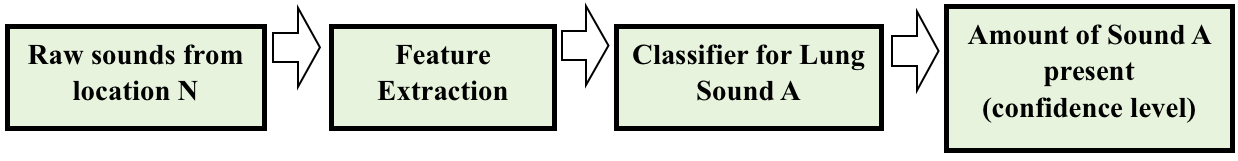
\includegraphics[width=\linewidth]{images/SoftwareGoal1.png}
 	\caption{Software goal 1}
 \endminipage\hfill
 \end{figure}
 
 This section of software applied pattern recognition algorithms and machine learning to estimate how much of each type of lung sound is present in the sample sound file.  Since the amount of lung sound present is generally a subjective assessment performed by a human doctor, this portion of software involves its own machine learning algorithm to produce outputs in the form of estimates (confidence levels).  This software can be tested and validated separately against the results from a trained pulmonologist.\\
 
 Once we have calculated the amount of specific lung sounds present in each sample, from each location on the body, a second machine learning algorithm can be applied to perform the actual diagnosis.  This is shown graphically below:\\
 
  \begin{figure}[H]
  \minipage{\textwidth}
  	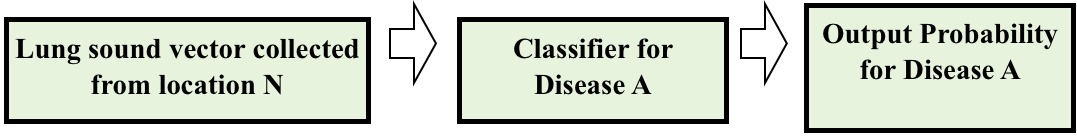
\includegraphics[width=\linewidth]{images/SoftwareGoal2.png}
  	\caption{Software goal 2}
  \endminipage\hfill
  \end{figure}

  For this UAP project, I am focusing on Part 1 of the software, with the goal of identifying the amount of each lung sound present in the sound files.\\
  
\section{Lung Sounds}

There are traditionally 3 types of lung sounds used in the diagnosis of pulmonary disease: wheeze, crackle, and pleural rub. 

\subsection{Wheeze}

Wheeze is characterized by a set of continuous sounds, sometimes described as “musical” which is produced by restricted air flow when the person inhales and exhales.  Multiple frequencies can be heard in these sounds.  More recently, several clinical organizations have divided the wheeze category of sounds into two separate categories: high-frequency wheeze and low-frequency wheeze, in order to differentiate between the characteristic wheezing produce by the upper and lower parts of the respiratory system, respectively. (see reference online).

\subsection{Crackle}

Crackle

\subsection{Pleural Rub}

Pleural Rub

\section{Software Implementation}

\subsection{Software Tools}

 With the goal of machine learning classification in mind, the first task was to determine what tools were to be used on the lung data. \\
 
 The most fundamental function of the application is for machine learning algorithms to give a binary classification of the data, ie. either the patient has the disease or the patient does not suffer from the disease. Since these classifiers only state "yes or no" instead of "which", each disease will require its own classifier. The most common technique for this type of classification is a simple linear classifier called a support vector machine (SVM). The SVM will train on pre-classified data of Indian patients with the target diseases and aims to minimize potential misclassification of future patients based off of the sample data. Since there are no known machine learning libraries for Android devices a large portion of the work for this project will be in the implementation, training, and testing of these algorithms.\\
 
 I investigated several machine learning libraries available in Java including: Weka, Mallet, and LibSVM. Each of the options, however, had drawbacks that were cause for hesitation. Weka is a comprehensive suite of machine learning algorithms and data mining tools. The software is one of the most popular machine learning packages available and is available into both an executable form to run on pre-formatted data as well as a developers version that can be modified for specific needs. Unfortunately the documentation for the software was rather difficult to traverse and contained a large host of functionalities that both were outside of the scope of the needs of classification and outside of my knowledge in machine learning. Since the timescale for this project was so limited, I wanted to minimize the ramp up time of learning and integrating a complex library, which made this option unattractive. Additionally investigation revealed that potential issues would arise in porting the Weka code to Android, so the long-term use of the software was in question. Mallet was attractive initially because its documentation was more comprehensible and easier to navigate than that Weka provided. However it advertises itself as a package for natural language processing and document classification, which is a large field utilizing techniques not necessarily applicable to the lung sound data. The final consideration, LibSVM, is Java software ported from a popular C package of the same name. Therefore the limited supporting documentation was written in C, which I have no experience with, and had difficulty parsing.\\
 
 The lack of clear documentation, potential trouble in porting from Java to Android, and concerns over underutilization of the software features at a great cost to system resources called into question the benefit of using a machine learning library. I had implemented classification algorithm’s before in a machine learning course I was concurrently enrolled in and pushed forward the idea of doing the algorithms myself for this project. This involved three steps: creating a working classifier, implementing the SVM algorithm, and running classifications on lung data.\\
 
 My first task was to implement the perceptron algorithm – a simple, but widely used classifier. I had written this before in Python for use in classification of data from Twitter, so conversion to Java was relatively straightforward. The Java implementation was ran on the same Twitter data as a check for correctness, since the performance should have been comparable to the Python code. In regards to the classifier itself the only challenge was performance. The mathematics behind the algorithm is heavily dependent upon multidimensional matrix manipulations. Traditional looping constructs, although viable for correctness, would have yielded a product virtually unusable due to computation time. The Python code addressed this by using the Numpy library. I researched for a comparable linear algebra toolkit in Java and settled on The Apache Commons Mathematics Library. With efficient matricies at hand, I wrote several parsers for formatting the Twitter data and extracting features to classify on. The classifier was tested on a pre-labeled set of test tweets and correctly labeled over 85\% of the points. Thus a basic classifier was available for any data set.\\
 
 The code was structured so that pieces may be swapped out easily. The three main components were the parsers to read in data, algorithms to construct a feature matrix from the data, and the machine learning algorithm to classify the data. The second task was to implement a more powerful classifier – a SVM. The SVM algorithm is similar to perceptron in that they are both linear classifiers. The advantage of the SVM, however, is that it is a maximum margin separator. This means that the classification line will pass through the point that maximizes the distance between the nearest oppositely labeled training data points. If the line passed closer to one of the data points, then the likelihood that the classifier overfits the data increases. Overfitting gives good results on testing data but has the tendency to generalize poorly to test data in the general population.\\
 
 At this stage SVMs had just been covered in the machine learning course. The techiques for implementing a SVM were very different from the perceptron algorithm and required linear solvers. It became apparent that implementing this myself was not optimal because it would have required yet another library to be brought in to the project and forseeably a great undertaking in working out all of the details of the algorithm. Thus I decided to turn back to incorporating a machine learning library, specifically LibSVM. The modular structure of the existing code made integration of the library’s SVM classifier a smooth process with minimal changes. With a SVM in hand the focus of the project switched to classification on the lung data. (include SVM confidence interval)

\subsection{Feature Extraction}

Feature extraction is the most open ended and challenging  component of the project. Since Android devices have limited processing power due to their mobile processing cores a balance was struck between having enough features to be able to separate lung conditions while keeping computational demand at a minimum. The features should not only correctly classify lung sounds, but also do so with a high degree of confidence. \\

\begin{figure}[h!]
	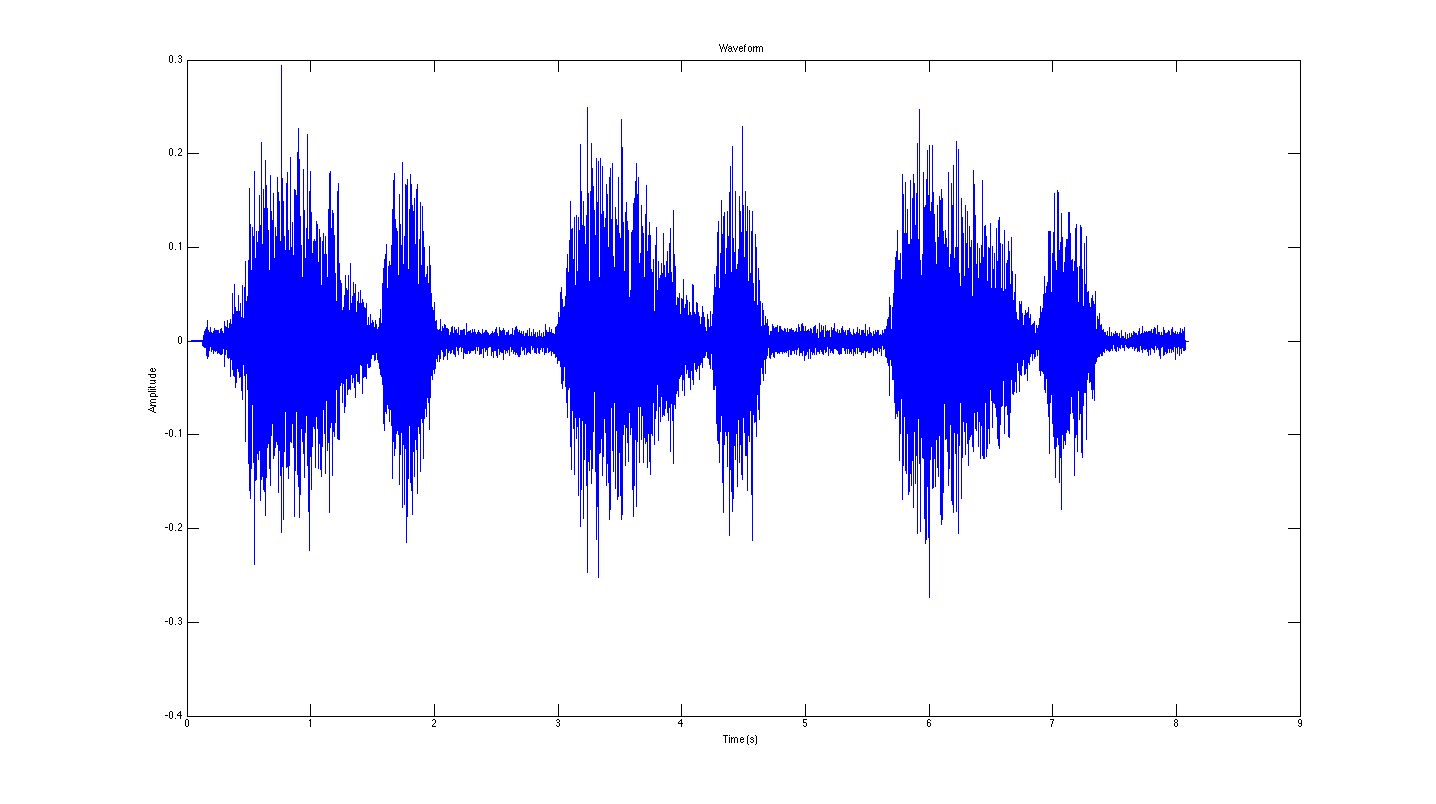
\includegraphics[width=\linewidth]{images/VesicularWaveform.png}
	\caption{Waveform of vesicular lung sound}
 	\label{fig:VesicularWaveform}
\end{figure}

Lung data comes in the form of an audio file represented by an of signal amplitude taken at regular intervals determined by the sampling frequency. A graph of amplitude over time represents the waveform of the lung sound, as seen in Figure \ref{fig:VesicularWaveform}. From the waveform one can see the cycles of inhalation and exhalation, which are the pairs of high amplitude signals separated by low amplitude lulls between breaths. \\

\subsubsection{Wheeze}

\paragraph{Characteristics}

Lung wheeze is characterized by well-defined pitches over sustained durations. To observe the pitch characteristics the signal is tranformed from the time domain to the frequency domain through a Fast Fourier Transform. Clinicians categorize wheeze into two types: low wheeze and high wheeze. These wheezes, respectively, have large magnitude peaks in low frequency (<200 Hz) and higher fequency regions. Figure \ref{fig:FFTVesicularWheeze} overlays a vesicular and high pitch wheeze in the frequency domain. The low frequency portions of each signal do not show an appreciable difference in magnitude. The high frequency signal magnitudes, on the other hand, differ greatly. The vesicular signal has a gradual and relatively constant decrease in magnitude moving into the higher frequencies. The wheeze signal instead has a very large magnitude peak that is approximately four times greater than strongest frequency signal of the vesicular data. \\

\begin{figure}[H]
	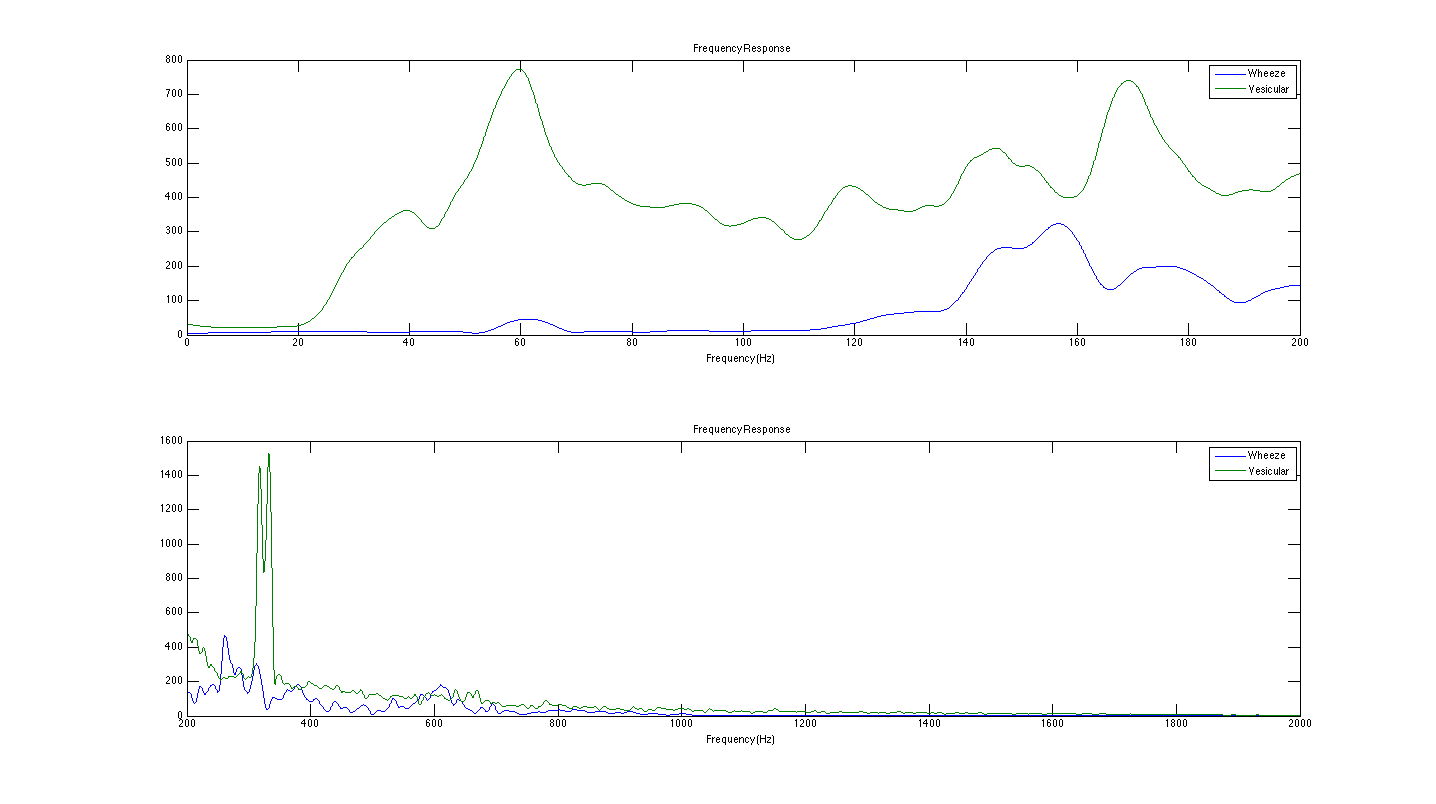
\includegraphics[width=\linewidth]{images/FFTVesicularWheeze.png}
	\caption{Comparison of vesicular and high pitched wheeze in frequency domain}
 	\label{fig:FFTVesicularWheeze}
\end{figure}

\paragraph{Sliding Window Count}

Wheeze characteristics are not uniform across the signal, so the time domain signal is discretized into 300ms blocks for detection of these characteristics. The technique for identifying wheeze components of a lung sound was drawn from the wheeze detector algorithm of \cite{Yi MEng}. A 300ms window was chosen because The American Thoracic Society defines the minimum duration of a wheeze to be 250ms, so this window should encapsulate the entire waveform with tolerance for deviation from the average. One can visually identify the wheeze by the regular periodic nature of the signal in the time domain. The frequency of signal over these spans is the fundamental frequency, which is the frequency at which a large spike will appear in the frequency domain. An example of the regular nature of the wheeze component is seen in Figure \ref{fig:WheezePeriodicity}. This contrasts sharply with the random and irregular progression of time domain signals for non-wheeze components of a wheeze signal and the entire signal span for other lung sounds, as seen in Figure \ref{fig:WheezeRandomness}. Note that these come from the same signal and are only seperated by approximately a 500ms duration. \\

\begin{figure}[H]
	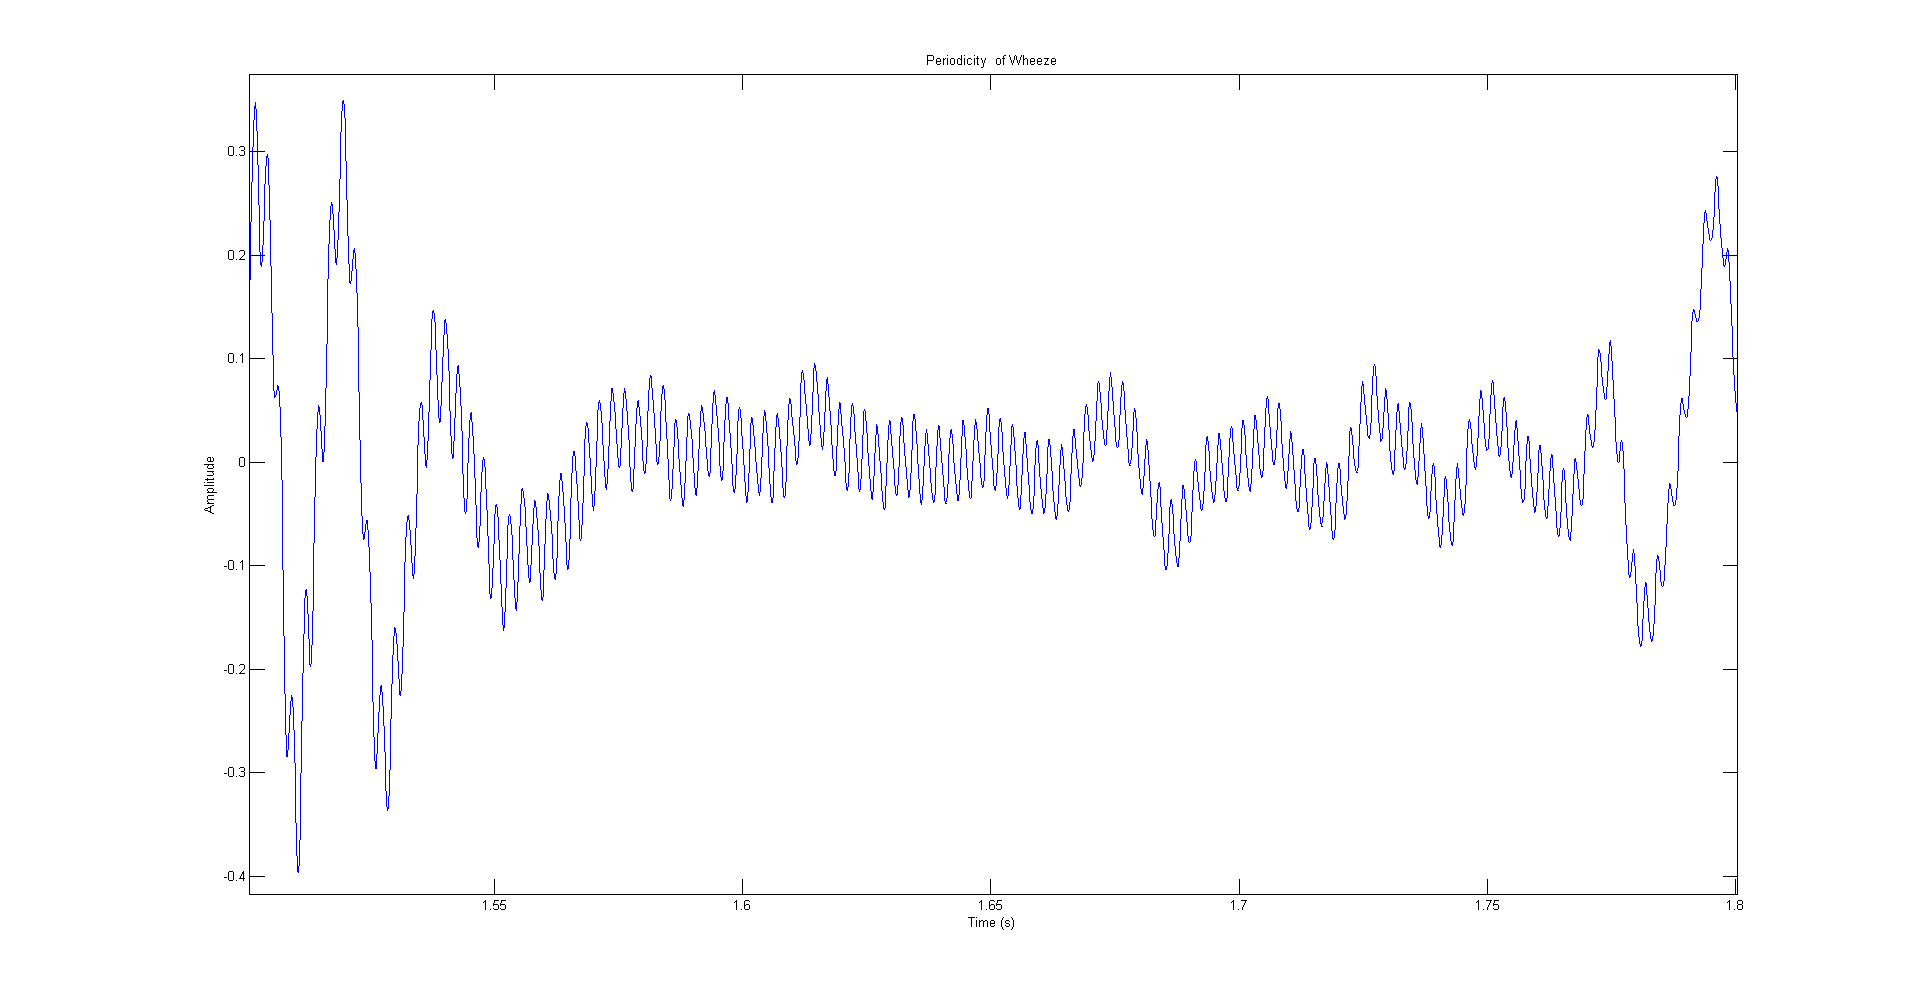
\includegraphics[width=\linewidth]{images/WheezePeriodicity.png}
	\caption{Wheeze component of time domain signal}
 	\label{fig:WheezePeriodicity}
\end{figure}
\begin{figure}[H]
	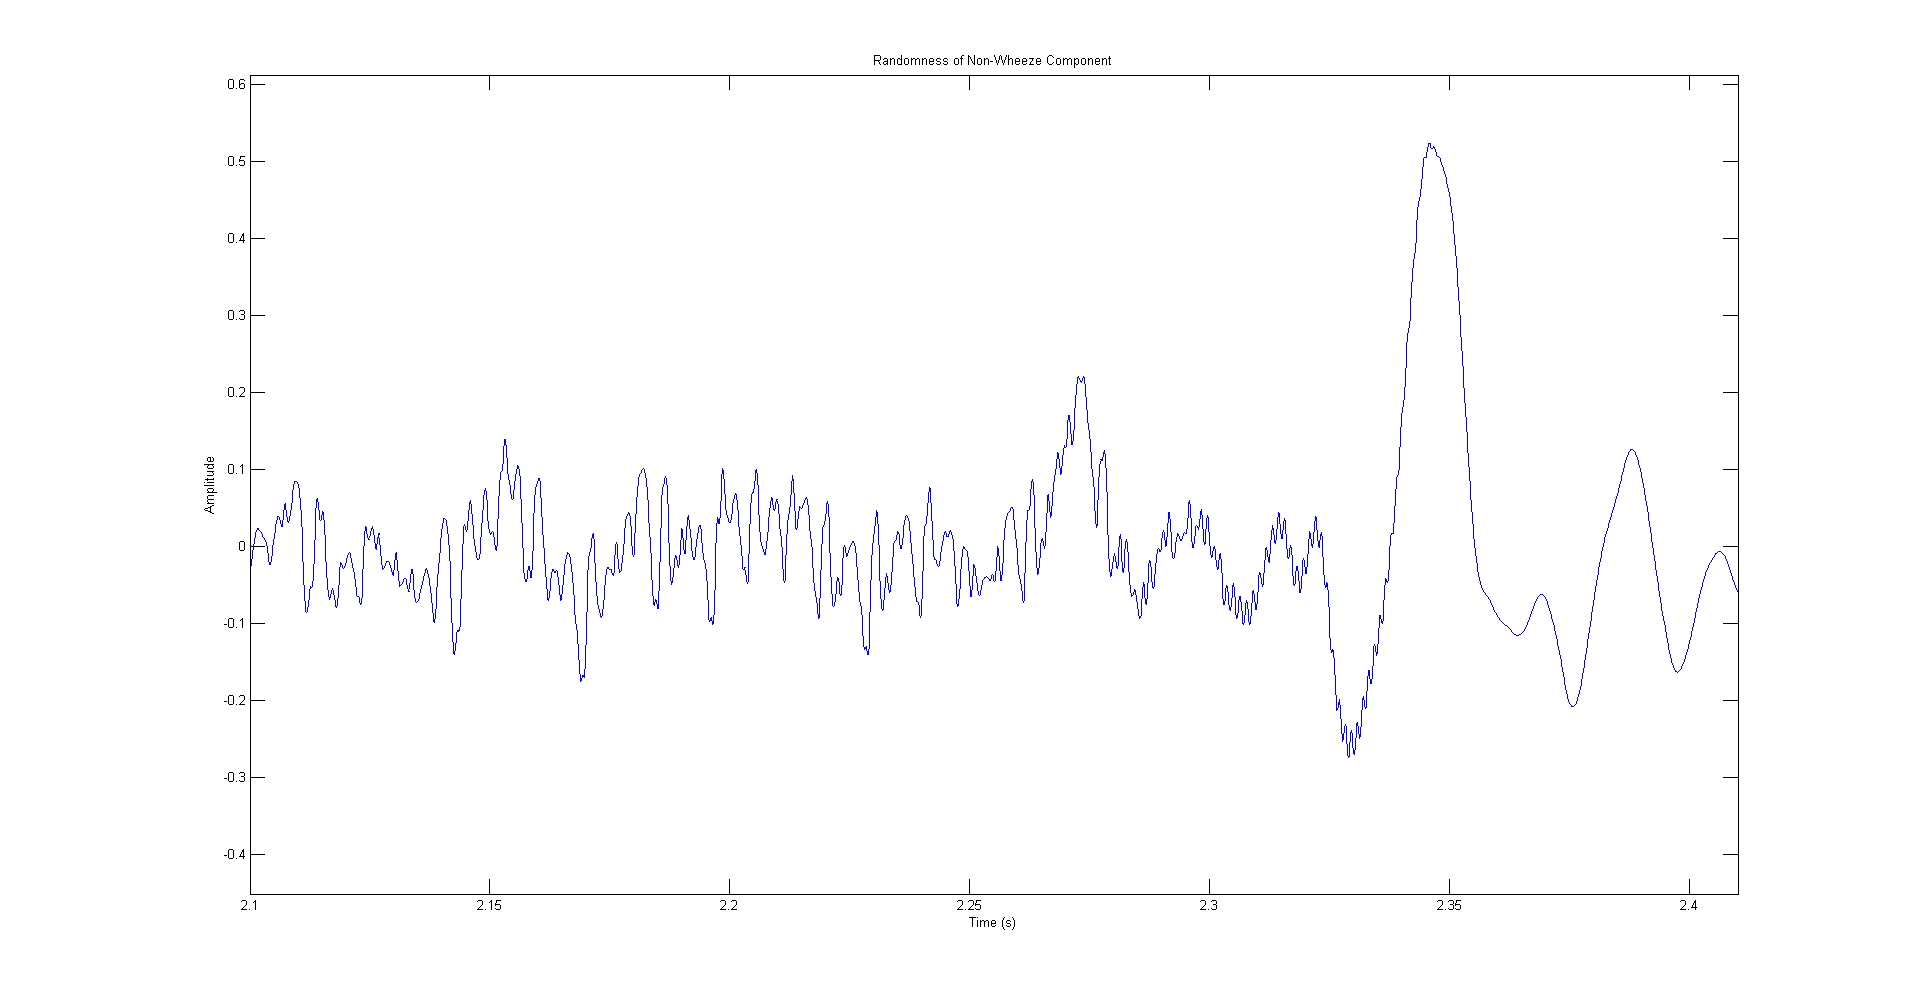
\includegraphics[width=\linewidth]{images/WheezeRandomness.png}
	\caption{Non-wheeze component of time domain signal}
 	\label{fig:WheezeRandomness}
\end{figure}

In each window the time domain signal is tranformed into the frequency domain., smoothed for noise reduction, and...\\

\subsubsection{Features}

\begin{itemize}
\item
	Peak frequency in low frequency region (<200 Hz)\\
	Capture magnitude of spike of low frequency wheeze\\
\item
	Peak frequency in middle frequency region (200-800 Hz)\\
	Capture magnitude of spike of high frequency wheeze\\
\item
	Peak frequency in high frequency region (>800 Hz)\\
	Capture magnitude of spike of high frequency wheeze\\
\item
	Ratio of max signal amplitude in low frequency region to average signal amplitude in low frequency region\\
	Capture a spike of low wheeze, which should have a high maximum to average magnitude ratio, and normalizes across different signals\\
\item
	Ratio of max signal amplitude in middle frequency region to average signal amplitude in middle frequency region\\
	Capture a spike of high wheeze, which should have a high maximum to average magnitude ratio, and normalizes across different signals\\
\item
	Ratio of signal amplitudes across low frequency region to middle frequency region\\
	(Explanation)\\
\item
	Ratio of signal amplitudes across high frequency region to middle frequency region\\
	(Explanation)\\
\end{itemize}

\subsubsection{Crackle}

The following features are extracted to characterize crackle, with the motivations behind choosing each feature: \\

\begin{itemize}
\item
	Ratio of signal amplitudes across low frequency region to middle frequency region\\
	(Explanation)\\
\item
	Ratio of signal amplitudes across high frequency region to middle frequency region\\
	(Explanation)\\
\end{itemize}

\section{Results}

\section{Conclusion and Future Work}

\newpage

\begin{thebibliography}{9}

\bibitem{Yi MEng}
	Yi, Gina A., and John V. Guttag. A Software Toolkit for Acoustic Respiratory Analysis. Thesis. Massachusetts Institute of Technology, 2004. Cambridge: Massachusetts Institute of Technology Libraries, 2005. DSpace@MIT. Massachusetts Institute of Technology. Dept. of Electrical Engineering and Computer Science. Web. 01 Apr. 2014.
\bibitem{Speech Analysis}
	"Lecture 10: Speech Signal Analysis." Introduction to Computer Programming with MATLAB. UCL Department of Phonetics and Linguistics, n.d. Web. 01 Apr. 2014.

\end{thebibliography}

\end{document}